\begin{figure}[H]
	\begin{center}
		  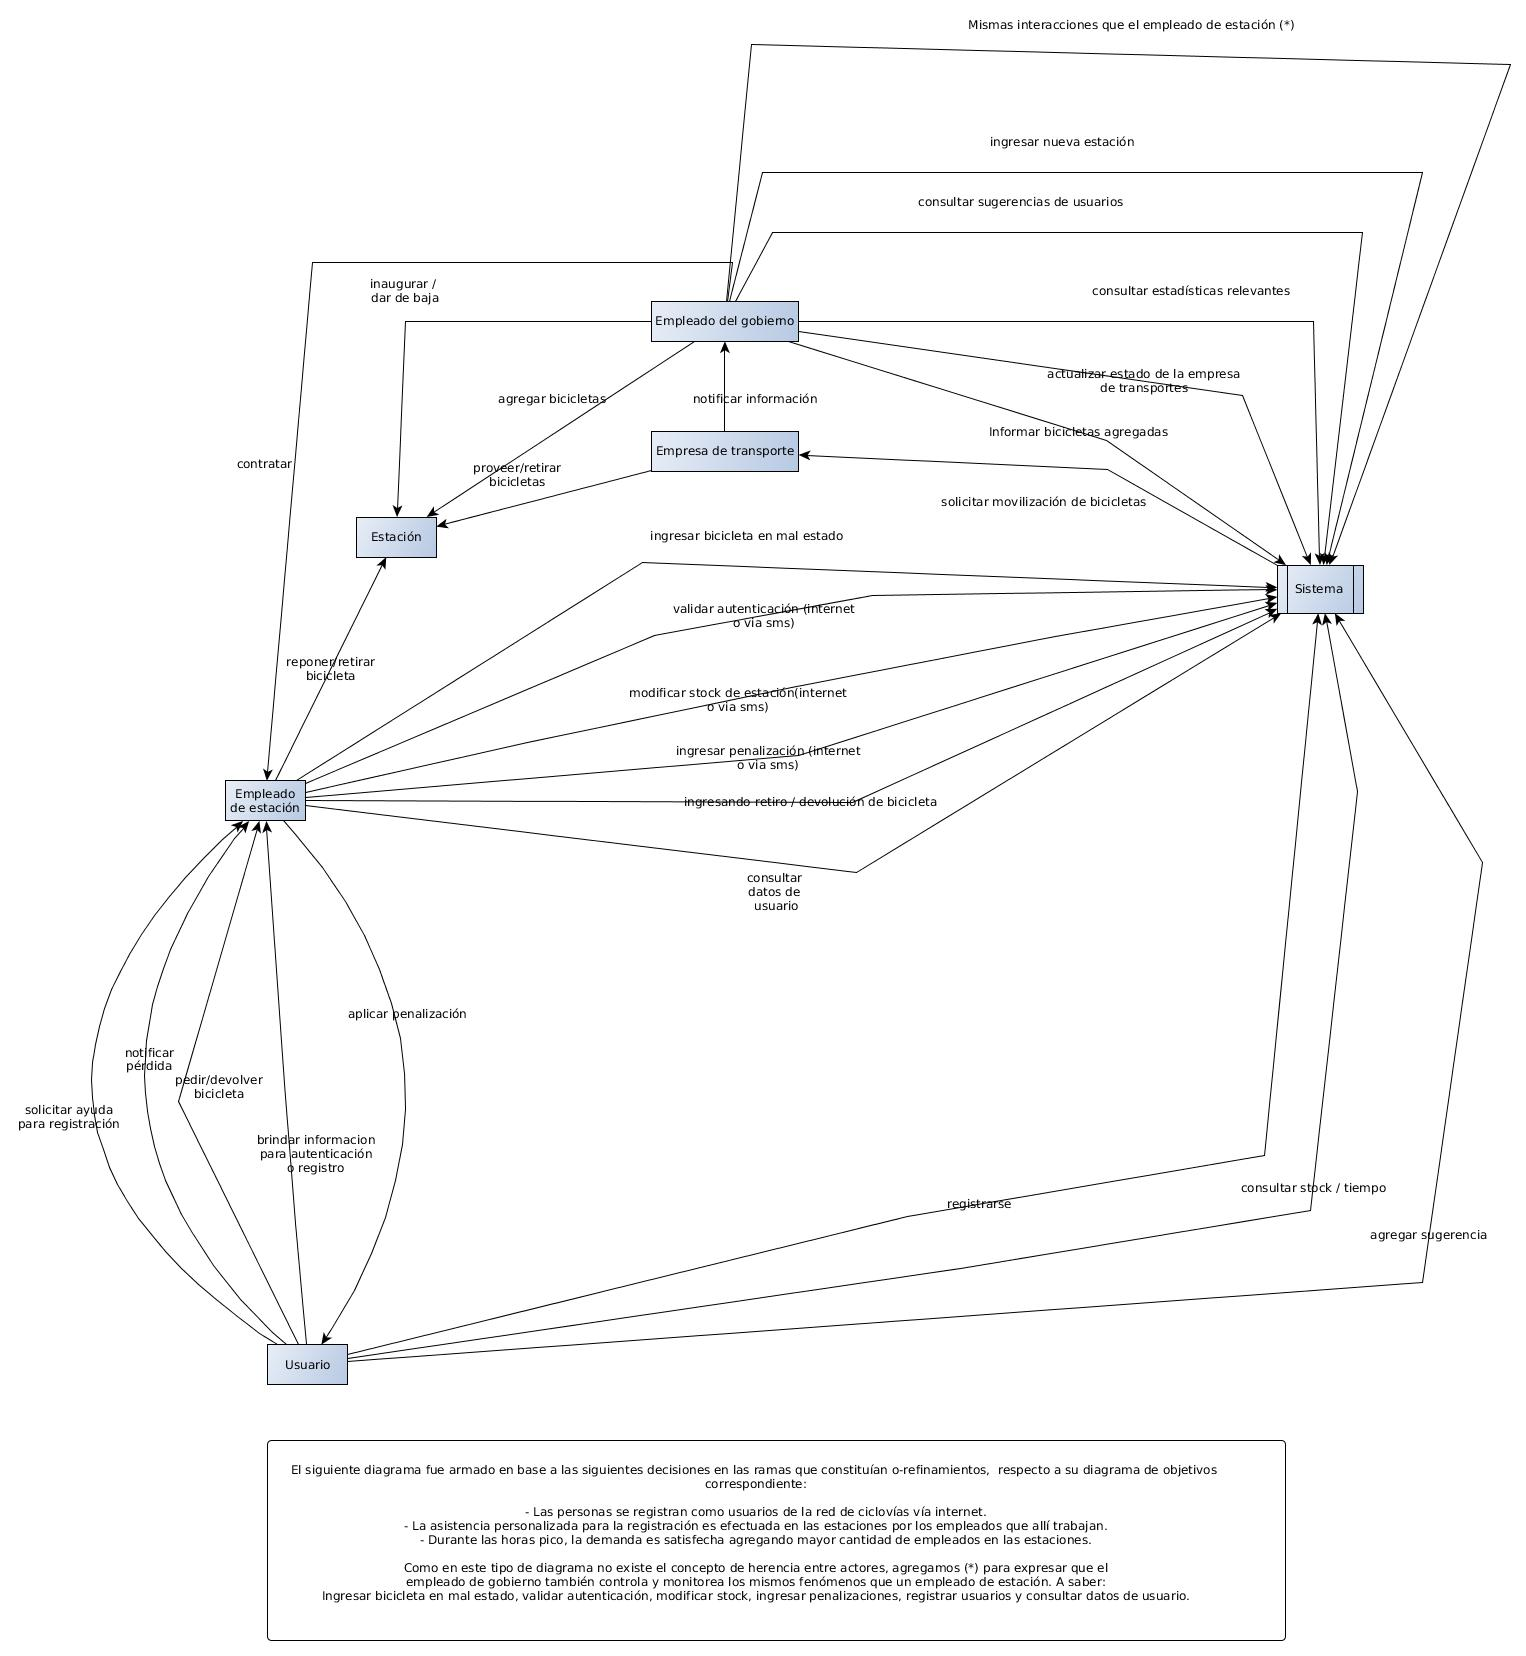
\includegraphics[scale=0.35]{diagrama_contexto.jpg}
		  \caption{}
		  \label{fig:contra1}
	\end{center}
\end{figure}

Los eventos relacionados con nuestra red de ciclovías son controlados y monitoreados por distintos agentes. Cada uno de ellos cumple una función única dentro del mismo.
Los usuarios comienzan registrándose por internet brindando los datos requeridos. Entre ellos se destacan principalmente el nùmero de DNI y el nombre completo, ya que ambos serán utilizados
para validar la identidad cada vez que quieran hacer uso de la red. En el caso de tener dificultades para completar este proceso puede acercarse a una de las estaciones y solicitar ayuda a uno de los empleados.
Siempre que un usuario quiera acercarse a una estacion para retirar una bicicleta tiene la opción de consultar previamente la disponibilidad de stock. En caso de estar agotado, el sistema informará el tiempo
estimado en el cual se repondrá el stock.
